\section{Empirical Results}
\label{sec:results}
We first report overall outcomes and progress (RQ1), then examine differences across phases and vulnerability classes (RQ2), and finally characterize recurring failure modes (RQ3). The numerical tables and curves retain the original scoring outputs. They are interpreted as historical measurements under the rubric, with the specific reconciliation and target-validation limitations stated below.




\subsection{Overall Outcomes and Progress (RQ1)}
% All statistics in this section use best-of-three (max per CVE-model pair across 3 runs) -> per-pair average.
Table~\ref{tab:model-results} reports the best-of-three results for each model across 30 CVEs. \texttt{glm-5.2} achieves the highest average overall score (64.6/100), followed by \texttt{mimo-v2.5} (52.9) and \texttt{claude-sonnet-4.6} (50.0). Under the original rubric, 11 of 150 CVE--model pairs achieve near-full P5 credit ($\geq$15/20), while 8 achieve near-full P6 credit. These thresholds describe historical scores, not independently adjudicated end-to-end success.


Historical item annotations identify 16 candidate runs across eight CVE--model groups and five CVEs. The old manuscript describes three execution strategies among these records; target identity, effects, and entry-path scope remain subject to AUD-01. Firstly, same-architecture \textit{chroot} on CVE-2023-26315 (AArch64) enables 6 runs---\texttt{claude-sonnet-4.6} twice, \texttt{deepseek-v4-flash} once, and \texttt{glm-5.2} three times---where the host and target share the same instruction set and no emulation is needed. Secondly, QEMU system mode with MikroTik's CHR image on CVE-2025-6443 enables 6 runs---\texttt{glm-5.2} three times and \texttt{gpt-5.5} three times---where the agent boots the full OS, sends crafted VXLAN packets, and records evidence interpreted as an access-control bypass via packet sniffer evidence. Thirdly, FastCGI socket injection with LD\_PRELOAD stubs on CVE-2023-44418, CVE-2024-5293, and CVE-2020-13389 enables 4 runs by \texttt{glm-5.2}, where the agent builds NVRAM/nofork stub libraries, launches the real \texttt{prog.cgi} or \texttt{httpd} under QEMU user-mode, and triggers SIGSEGV crashes or return-address overwrites on the real binary. In contrast, devices whose firmware is unavailable or requires complex cross-architecture emulation with proprietary NVRAM dependencies almost universally fail at P5.


The leading recorded configuration, \texttt{glm-5.2}, also shows stronger acquisition scores and fallback-plan scores. It averages 11.5/15 on P2 (Firmware Acquisition) under best-of-three scoring, well above \texttt{claude-sonnet-4.6}'s 7.7/15; since P2 gates all downstream phases, this gap cascades---in 5 out of 30 CVE--model pairs, \texttt{claude-sonnet-4.6}'s best plan exceeds 50 yet its best task stalls below 15, all blocked at P2. \texttt{glm-5.2} also achieves the strongest fallback planning (50.8/100 vs.\ 27.5--43.3 for the others), which correlates with deeper pipeline progression. The inspected examples connect continued acquisition attempts and alternative strategies to further progress. These associations do not isolate their causal contribution or an intrinsic property of the model.

Finally, we also report the computational cost of each model in our appendix, including per-run token consumption, API cost, and execution time across all 450 runs.

\subsection{Phase-Level Progress and Contrasting Cases (RQ2)}
%%% RQ6: graded评分揭示二元评分隐藏的差异
%%While 143/150 pairs (95.3\%) would be failures under binary %%evaluation, graded scoring reveals a 23.5-point spread (41.7--65.%%2). Best-of-three scoring adds $\sim$10 points over per-run %%averages, with stronger models showing larger variance (e.g., %%\texttt{glm-5.2}: +14.3), suggesting that succeeding at least once %%is itself a capability dimension.
%%

\begin{figure*}[t]
    \centering
    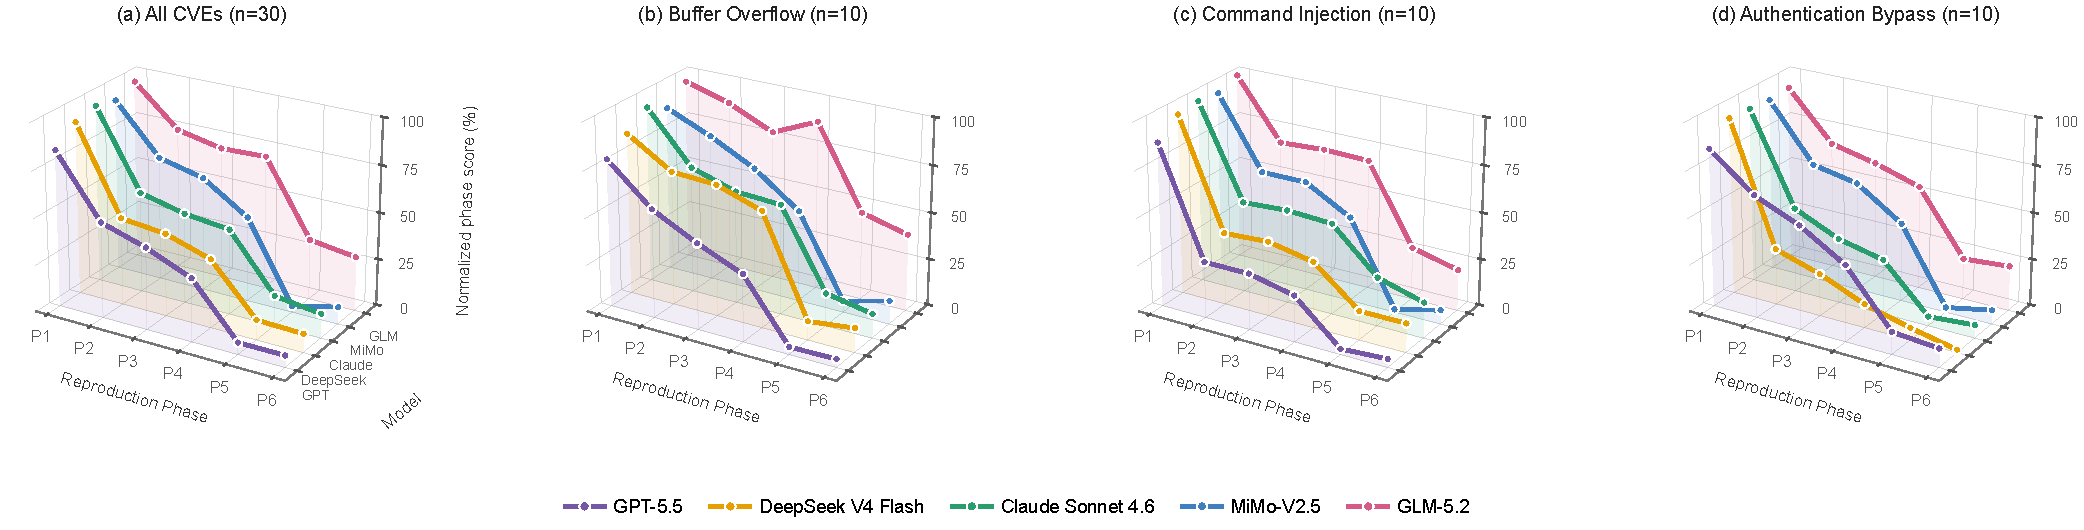
\includegraphics[width=\textwidth]{figures/3d.pdf}
    \caption{Normalized phase scores across model configurations, retaining the original best-of-three aggregation. Heights are score fractions, not completion or success rates; adjacent phase values need not come from the same trial.}
    \label{fig:heatmap}
\end{figure*}

% 异常点分析：19个CVE存在分化，graded评分暴露阶段特定能力
To examine distinctions not represented by a binary outcome, we conduct an anomaly analysis across all 450 runs. We define a \textit{divergence point} where a minority of runs score $\geq$50\% of the phase maximum while a majority score $<$25\%. These two thresholds are chosen to separate higher artifact credit from the small attempt-score contribution, which caps at $\sim$7\%. For each CVE we select the earliest divergent phase to avoid cascading low scores from unmet prerequisites. We identify 19 scoring results that exhibit such divergence and inspect the \textit{high} and \textit{low} runs' artifacts and trajectories for each. The divergence concentrates at P2 (firmware acquisition, 12/19), P4 (binary identification, 2/19) and P5 (service rehosting, 5/19). The retained contrasting cases illustrate three kinds of behavior associated with different phase scores. These examples do not estimate the effect of intervening on those behaviors.

% 三大分化模式：阶段特定能力
\noindent{\textbf{PSC 1: Search Strategy.}} The first divergence point is whether the agent verifies the assumption that firmware is unavailable, written in the plan. High runs test the ``firmware unavailable'' hypothesis by issuing real \texttt{curl} requests to vendor CDNs, regional sites, and community firmware archives. However, low runs just accept the hypothesis without verification and jump to simulation. For example, on CVE-2020-14140, only one of 15 runs actually curls the Xiaomi CDN, discovers the firmware is publicly downloadable, and statically analyzes the extracted Lua controllers; the other 14 runs assume unavailability and produce Python mock servers with zero \texttt{curl} invocations.

\noindent{\textbf{PSC 2: Tooling Knowledge.}} When firmware is encrypted in a vendor-proprietary format, standard \texttt{binwalk} fails and the agent must find out the correct decryption tool. High runs possess domain-specific tooling knowledge to handle encrypted firmware. For example, the \texttt{delink} tool is used for D-Link MH01 encryption, and the correct SHRS decryption key recovered from a sibling model (DIR-3060) is used for DIR-X3260 firmware. However, the low runs assume standard \texttt{binwalk -e} suffices and produce empty extraction. On CVE-2024-6045, only 4/15 runs know the \texttt{delink} tool is required; low runs create empty directories because the default tool cannot process MH01 encryption.

\noindent{\textbf{PSC 3: Rehosting Technique.}} Even with the correct binary extracted, proprietary firmware services fail under QEMU due to missing NVRAM state, kernel ioctl dependencies, and non-standard FastCGI interfaces. High runs employ techniques such as QEMU \texttt{-L} sysroot for library resolution, LD\_PRELOAD NVRAM/nofork stubs, and direct FastCGI socket injection. Low runs hit QEMU failures and switch to C/Python reimplementation. For example, on CVE-2020-13389, the top run (\texttt{glm-5.2}, 19/20) uses QEMU \texttt{-L rootfs} to launch the real Tenda httpd, while a low run using \texttt{chroot} fails on \texttt{br0} ENODEV. On CVE-2023-44418, the top run (\texttt{glm-5.2}, 20/20) identifies \texttt{prog.cgi} as a FastCGI responder and injects protocol frames via a Unix socket; a run with full P1--P4 credit scores only P5=4 by treating it as a standalone web server.

%%Note that under binary evaluation all 19 divergent CVEs would be uniformly labeled as failures, yet the high runs demonstrate distinct capabilities---hypothesis verification, tool-chain selection, and environment engineering---that are directly transferable to real-world vulnerability analysis but invisible without graded, phase-level scoring.



% \begin{mdframed}[linecolor=black,linewidth=1pt,backgroundcolor=gray!10,roundcorner=3pt,nobreak=true]
% \noindent\textbf{Result-2:} Evidence-grounded scoring reveals distinctions hidden by binary success. Anomaly analysis exposes three phase-specific capabilities that can pass through the bottlenecks.
% \end{mdframed}

\subsection{Differences across Vulnerability Classes (RQ2)}



% Statistics: Overall score = best-of-three -> per-pair average.
% Phase-level numbers (P2, P4) and FW% = per-run average across 150 runs per class.
% CVE-level best scores (e.g., 99.0, 80.8) = best-of-three -> max across pairs and models.
We disaggregate the 450 runs by vulnerability class. The three classes differ in best-of-three overall score (58.5 vs.\ 48.9 vs.\ 46.0 for BOF, CMDI, and AUTH respectively), but the more striking differences lie in \emph{where} the pipeline breaks for each class.


\noindent\textbf{Buffer Overflow} performs best across the early phases. Agents average 8.06/15 on P2 (Firmware Acquisition) and 7.09/15 on P4 (Binary Identification), and 73\% of runs acquire the firmware. In the selected cases these values exceed those in the other classes. Some overflow descriptions expose a concrete function-level target (\texttt{strcpy}/\texttt{sprintf} on a named binary), so agents can confirm the vulnerable code path by grepping for the function name in the extracted binary, yielding high P4 scores. For CVE-2023-41229 and CVE-2023-44418 (D-Link \texttt{prog.cgi}), agents identify the HNAP Referer vector and target binary upfront, providing concrete targets for the firmware analysis. This observation does not establish why an agent chose original-target execution over simulation.


\noindent\textbf{Command Injection} shows the sharpest polarization. It attains a 3.3\% high-trigger-score fraction (5/150 runs reaching P6$\geq$18) yet also a high simulation rate. Once a service is rehosted, shell side effects such as \texttt{uid=0} or file creation provide candidate evidence, but attribution to the original target still requires verification (e.g., runs on CVE-2023-26315 rehost the Xiaomi \texttt{plugincenter} via \texttt{chroot} and trigger root RCE). The bottleneck is acquisition: 50\% of command-injection runs stall after information gathering (P2--P6 all zero), as agents judge the vulnerability to require physical hardware and skip directly to Python simulation. The retained simulations can demonstrate command-injection logic with Python code. Their presence alone does not establish the agent's motivation or prove that original-target acquisition was impossible. Two CVEs form a low-score cluster (Overall $\leq$33) where almost no run acquires firmware---both involve non-standard services with dead or region-locked download URLs.


\noindent\textbf{Authentication Bypass} is weakest in binary identification (P4: 3.14/15 per-run average) and rehosting attempts. Its root cause is usually cross-component session or access-control logic rather than a single faulty function, so agents struggle to localize the vulnerable path in one binary---unlike buffer overflows where \texttt{strcpy} is directly greppable, an absent authorization check generally requires analysis beyond matching a function name (e.g., CVE-2021-33044's \texttt{clientType: "NetKeyboard"} parameter; CVE-2025-6443's VXLAN network-layer control). Trigger verification is also hard: unlike a crash or a command side effect, an auth-bypass requires a controlled authenticated and unauthenticated comparison.
%The exception is network-layer bypasses---CVE-2025-6443 (MikroTik) is fully reproduced by booting a RouterOS CHR image under QEMU system mode and sending VXLAN packets, bypassing binary-level analysis entirely.

Across the selected classes, phase scores and inspected examples differ in acquisition, component identification, and rehosting. Firmware availability, task descriptions, architecture, and vulnerability class co-vary, so the comparison does not isolate a causal effect of vulnerability semantics. P5 scores are low across the groups; low scores alone do not identify the most frequent observed stopping cause.
%---even BOF, the strongest, averages only 3.0/20---indicating that rehosting capability is the primary ceiling for LLM agents.
% regardless of vulnerability type.


%%\begin{mdframed}[linecolor=black,linewidth=1pt,%%backgroundcolor=gray!10,roundcorner=3pt,nobreak=true]
%%\noindent\textbf{Result-3:} Vulnerability class %%systematically shapes reproduction. Class differences %%couple to distinct rehosting paths, and firmware %%downloadability is the decisive external factor.
%%\end{mdframed}

\subsection{Failure Analysis (RQ3)}


\begin{figure}[t]
    \centering
    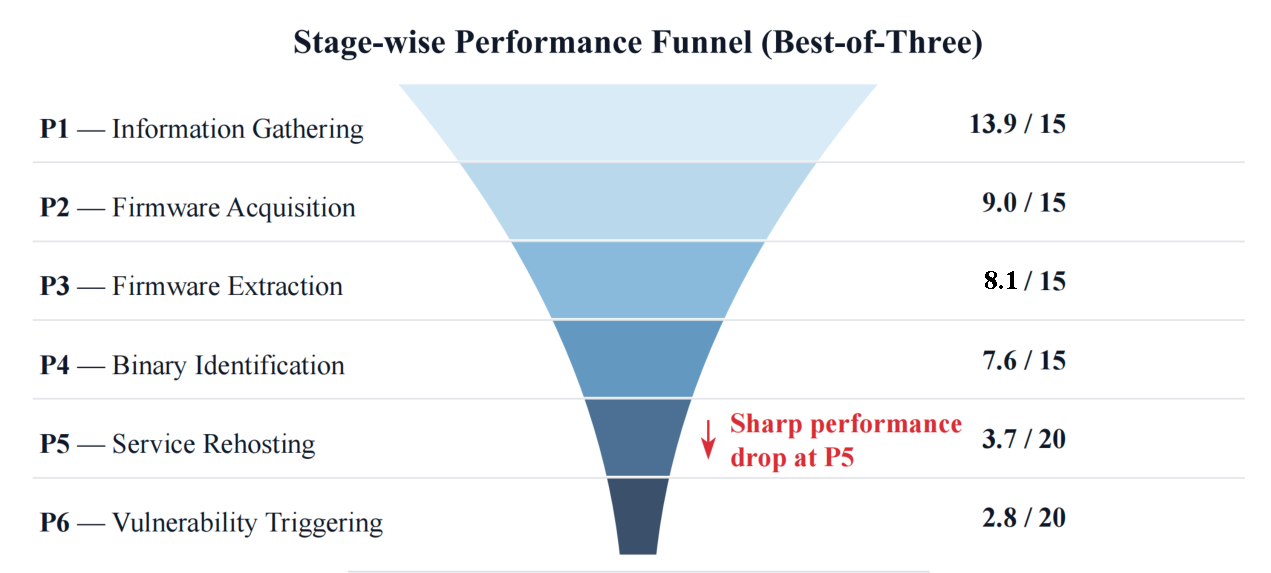
\includegraphics[width=0.45\textwidth]{figures/stagefunnel.pdf}
    \caption{Stage-level averages under best-of-three scoring.}
    \label{fig:stage-funnel}
\end{figure}


% RQ2: 阶段漏斗——P1-R4合理，R5骤降，terminal blocker主要在Phase 5
Figure~\ref{fig:stage-funnel} shows the stage funnel from P1 to P6. P1 (Information Gathering) is the strongest phase at 13.9/15, indicating high credit on the rubric's information-gathering items, without independently establishing fact correctness. P2--P4 show moderate scores, reflecting partial success in firmware acquisition, extraction, and binary identification. The sharp collapse occurs at P5 (Service Rehosting), which averages only 3.7/20. P6 averages 2.8/20, with most points coming from PoC construction rather than real-target triggering.

%%\begin{table}[t]
%%\setlength{\tabcolsep}{3.8pt}
%%\centering
%%\caption{Stage-level averages under %%best-of-three scoring. The pipeline %%collapses at P5.}
%%\label{tab:stage-funnel}
%%\renewcommand{\arraystretch}{1.15}
%%\begin{tabular}{c l r r r}
%%\toprule
%%\textbf{Phase} & \textbf%%{Description} & \textbf{Score} & %%\textbf{Max} & \textbf{\%} \\
%%\midrule
%%P1 & Information gathering   & 13.%%9 & 15 & 92.8\% \\
%%P2 & Firmware acquisition    &  9.%%0 & 15 & 59.9\% \\
%%P3 & Firmware extraction     &  8.%%1 & 15 & 53.8\% \\
%%P4 & Binary identification   &  7.%%6 & 15 & 50.8\% \\
%%\midrule
%%P5 & Service rehosting       &  3.%%7 & 20 & 18.6\% \\
%%P6 & Vulnerability triggering&  2.%%8 & 20 & 13.9\% \\
%%\bottomrule
%%\end{tabular}
%%\end{table}



% Failure attribution: per-run counts (terminal failure mode, each run counted once).
% P2/P5 blockers are terminal phase counts (TermPhase column).
Based on the sharp collapse and across all 450 runs,
%terminal blockers concentrate at two phases---P2 (211/450, firmware acquisition) and P5 (173/450, service rehosting)---consistent with the funnel above.
we analyze the dominant failure modes that drive these blockers:

\noindent{\textbf{Simulation substitution (legacy summary: 204/450, 45.3\%).}} The largest category in the legacy summary: agents produce mock servers, C harnesses, or host-native programs that demonstrate the vulnerability \emph{pattern} but not the target \emph{instance}. The output is often coherent and reproducible---valid crash signals, correct exploit syntax, convincing reports---yet never exercises the real firmware binary, so substitute-only demonstrations are ineligible for real-target execution credit. Explicitly declared simulation is distinguished from an unsupported success claim.

\noindent{\textbf{Rehosting gap (93/450, 20.7\%).}} Agents identify the target binary but cannot properly configure dynamic loaders, NVRAM values and abandon after one or two errors. Same-architecture (ARM64) devices bypass this gap, leaving cross-architecture (MIPS) targets that require QEMU emulation as the bulk of these blockers.

\noindent{\textbf{Firmware acquisition failures (75/450, 16.7\%).}} Agents fail to obtain the correct firmware image---downloading incorrect versions, stopping after 403 errors, or conflating firmware binaries with GPL source packages that lack runtime shared libraries.

\noindent{\textbf{Extraction failures (36/450, 8.0\%).}} Agents acquire firmware but misuse extraction tools---e.g., applying standard \texttt{binwalk} to vendor-encrypted images---or analyze binaries pulled from PoC repositories rather than from the target firmware.

\noindent{\textbf{Infrastructure failures (15/450, 3.3\%).}} The residual blockers stem from execution-environment setup rather than reproduction logic, and are scattered across phases rather than concentrated at any single stage.


\paragraph{Counting scope and reconciliation.}
The percentages above reproduce the legacy summary's terminal categories. An independent inventory of the current evaluator records finds 316 runs with any simulation label and 209 with at least one terminal simulation label; 11 runs have multiple terminal entries. These are different queries, not alternative validated prevalence estimates. \todo{NUM-01}{Reconcile 204 versus 209 terminal-simulation counts, source versions, and aggregation rules. Check category overlap and coverage before publishing a final failure distribution.} Neither a missing trace nor an evaluator's terminal label alone establishes the actual stopping cause.

